\section{Deskripsi Umum}

Penelitian ini bertujuan mengembangkan algoritma pembelajaran \textit{online} untuk skenario \textit{Iterated Prisoner's Dilemma} (IPD) dengan lawan reaktif deterministik. Fokus utama penelitian adalah pada pemodelan lawan multi-langkah rekursif. Model prediktif dilatih untuk mengestimasi distribusi aksi lawan berdasarkan riwayat interaksi, tanpa menggunakan informasi hasil sebagai sinyal pembelajaran. Model prediksi tersebut kemudian digunakan sebagai komponen dalam simulasi untuk mengestimasi nilai aksi agen. Penelitian ini diacu pada Gambar \ref{fig:AlurPenelitian} untuk ilustrasi alur penelitian secara keseluruhan.

\begin{figure}[!htbp]
    \centering
    \caption{Diagram metodologi.}\label{fig:AlurPenelitian}
    
\includegraphics[width=0.9\textwidth]{Images/AlurPenelitian.png}
\end{figure}

\section{Formulasi Masalah}

Penelitian ini menggunakan skenario \textit{Iterated Prisoner's Dilemma} (IPD) dengan panjang permainan tetap $T$. Untuk setiap episode permainan yang dinotasikan dengan indeks $n$, pada setiap giliran permainan $t = 1, \dots, T$, agen $i$ dan lawannya masing-masing memilih aksi aktual $a_{n,t,i}$ dan $a_{n,t,-i}$ yang berada pada himpunan aksi $\{C, D\}$. Hasil interaksi pada setiap langkah diperoleh berdasarkan matriks \textit{payoff} standar IPD. Lawan diasumsikan bersifat reaktif deterministik, sementara algoritma internal yang digunakan lawan tidak diketahui oleh agen. Agen tidak memiliki akses terhadap parameter internal, fungsi utilitas, maupun mekanisme pembelajaran lawan. Satu-satunya informasi yang tersedia bagi agen adalah riwayat interaksi hingga giliran ke-$t$ pada episode ke-$n$, yang dinotasikan sebagai $\mathcal{H}_{n,t} = \{(a_{n,1,i}, a_{n,1,-i}), \dots, (a_{n,t,i}, a_{n,t,-i})\}$.

Tujuan agen adalah memilih aksi pada setiap langkah permainan sehingga memaksimalkan hasil kumulatif sepanjang horizon permainan $T$. Untuk membantu proses pengambilan keputusan, agen memanfaatkan modul pemodelan lawan yang dilatih secara terpisah dari sinyal hasil interaksi. Modul ini menghasilkan distribusi prediktif atas aksi lawan pada langkah waktu berikutnya yang dinyatakan sebagai $P_\theta(a_{n,t+1,-i} \mid \mathcal{H}_{n,t})$, yaitu probabilitas aksi aktual lawan pada waktu target $t+1$ berdasarkan riwayat interaksi yang tersedia hingga waktu observasi $t$. Distribusi prediktif tersebut kemudian digunakan dalam mekanisme simulasi prediksi multi-langkah sepanjang horizon terbatas $H$, di mana model secara rekursif menghasilkan estimasi aksi lawan $\hat{a}_{n,t,h,-i}$ untuk setiap langkah prediksi ke-$h \in \{1,\dots,H\}$ guna memperkirakan konsekuensi jangka panjang dari aksi kandidat yang dipertimbangkan oleh agen.

Berdasarkan setting tersebut, penelitian ini bertujuan untuk menganalisis bagaimana penggunaan prediksi multi-langkah rekursif dalam interaksi closed-loop mempengaruhi akurasi pemodelan perilaku lawan serta stabilitas trajektori interaksi sepanjang horizon prediksi yang berbeda.

\section{Rancangan Algoritma Metode}
\subsection{Gambaran Umum}
Algoritma yang digunakan dalam penelitian ini menggunakan LSTM untuk memprediksi aksi lawan dalam horizon multi-langkah diperlihatkan pada gambar \ref{fig:AlurBesar}.
Metode dimulai dengan Spesifikasi lingkungan simulasi, menggunkan konfigurasi permainan berulang IPD. Antarmuka dapat menghasilkan riwayat permainan yang digunakan. Selanjutnya, dilakukan desain populasi strategi lawan yang mencakup berbagai tipe strategi untuk memastikan keberagaman dinamika interaksi. Prosedur simulasi generasi data dijalankan untuk menghasilkan trajektori interaksi antara agen dan lawan berdasarkan konfigurasi yang telah ditetapkan. Trajektori yang dihasilkan kemudian diproses dalam tahap representasi dan persiapan dataset. 

Setelah persiapan data selesai, dilakukan perancangan model prediksi lawan menggunakan arsitektur LSTM untuk menangkap dependensi temporal dalam interaksi dilakukan pembentukan komponen LSTM seperti forget gate, input gate, dan output gate. Kemudian Model akan dikembangkan lebih lanjut agar dapat melakukan prediksi multi-langkah menggunakan konsep rekursif.

Selanjutnya model dilatih menggunakan protokol pelatihan yang mencakup pelatihan satu langkah dan pelatihan multi-langkah. Pelatihan satu langkah akan menggunakan fungsi objektif cross entropy, sedangkan pelatihan multi-langkah akan menggunakan fungsi objektif Negative-log-likelihood atau NLL. NLL merupakan akumulasi cross-entropy sepanjang horizon dengan pembobotan Rank Order Centroid (ROC), langkah terdekat yang dihasilkan diberi bobot lebih besar dibanding langkah yang lebih jauh dan sebaliknya. 

Setelah model dilatih, dilakukan validasi model dengan melakukan hyperparameter tuning untuk memilih konfigurasi terbaik berdasarkan performa trajektorial, fungsi objektif yang dimaksimalkan adalah \textit{confusion matrix}.  

Setelah model terbaik dipilih, dilakukan pengujian model pada data uji untuk mengukur generalisasi akhir model terhadap distribusi yang tidak terlihat selama pelatihan. Pengujian dilakukan baik pada skenario strategi yang telah terlihat selama pelatihan maupun pada strategi yang sepenuhnya baru. Pengujian kemampuan generalisasi terhadap dinamika interaksi menggunakan \textit{confusion matrix} sebagai metrik evaluasi.

Interpretasi dan analisis terhadap hasil pengujian yang diperoleh dari eksperimen dan pembelajaran ablasi. Analisis difokuskan pada evaluasi akurasi pemodelan lawan dalam memprediksi aksi lawan pada horizon prediksi tertentu. Selain itu, analisis juga bertujuan mengidentifikasi komponen atau konfigurasi model yang berkontribusi terhadap peningkatan akurasi prediksi, seperti penggunaan riwayat interaksi, panjang horizon prediksi, serta variasi arsitektur model. 

Melalui analisis ini, dapat diamati sejauh mana setiap komponen mempengaruhi kualitas prediksi yang diukur menggunakan metrik evaluasi yang telah ditentukan.

\begin{figure}[!htbp]
    \centering
    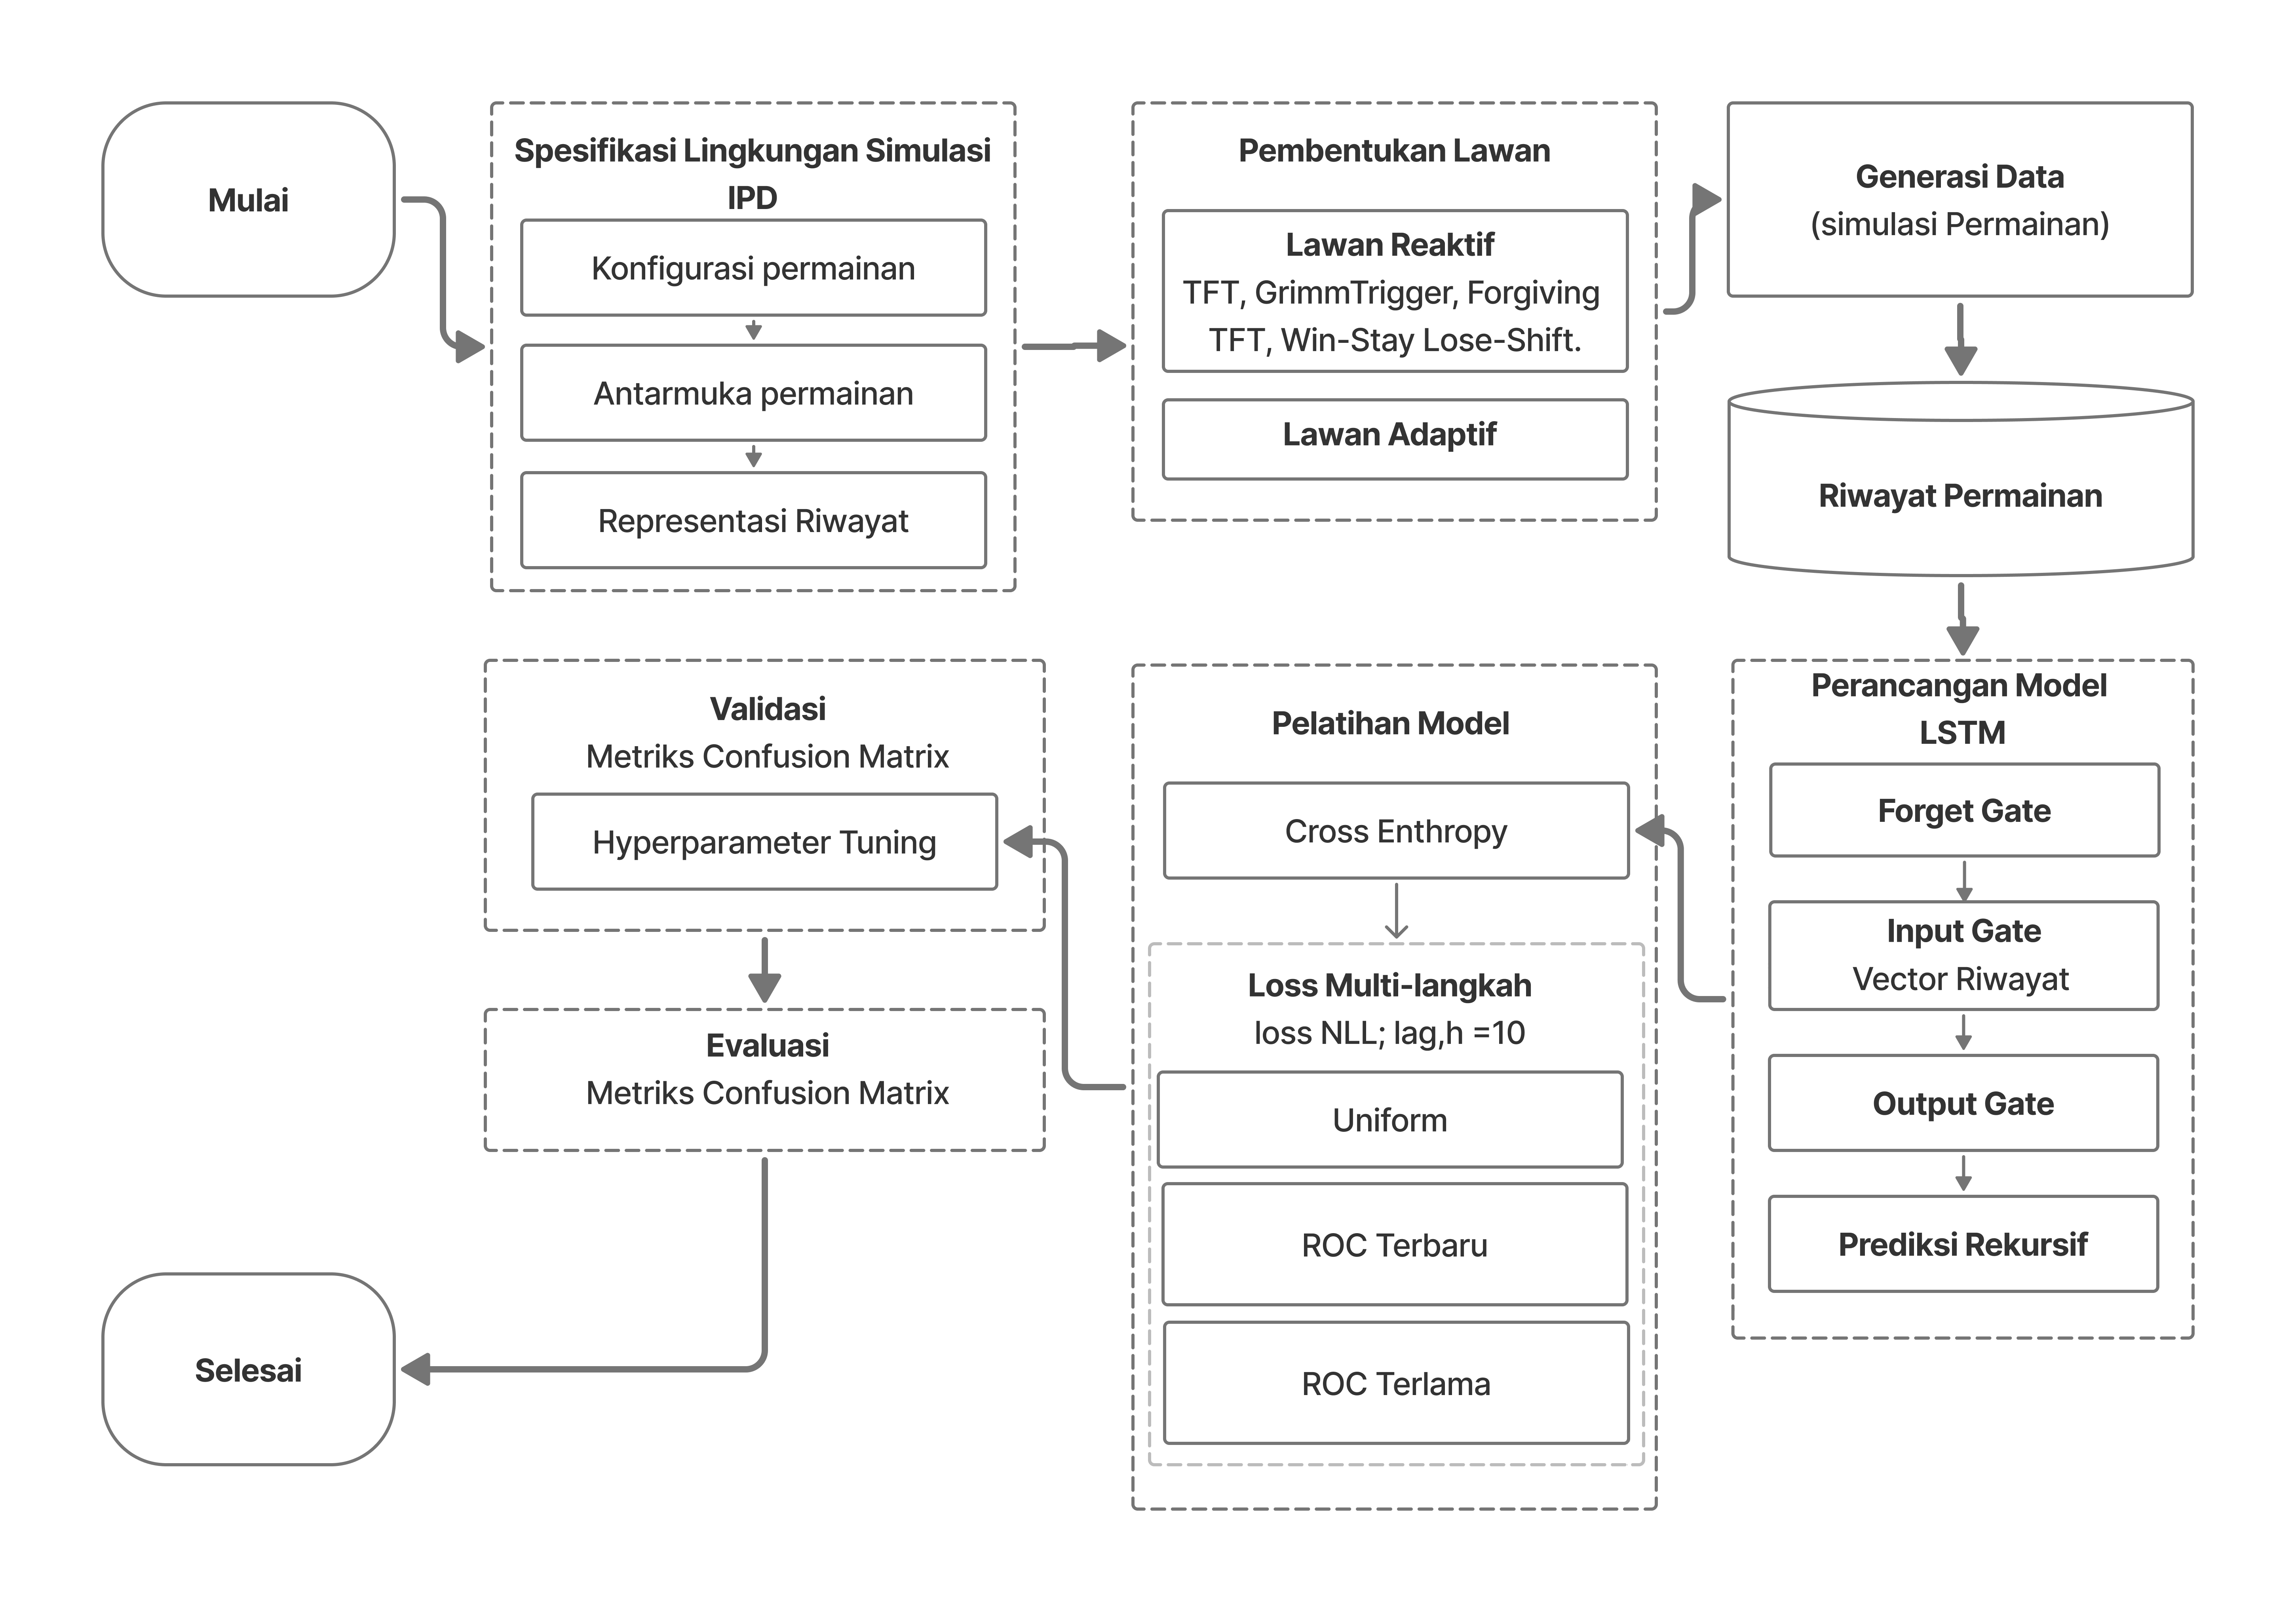
\includegraphics[width=0.8\textwidth]{Images/AlurBesar.png}
    \caption{Rancangan Algoritma Metode.}\label{fig:AlurBesar}
\end{figure}

\subsection{Spesifikasi Lingkungan Simulasi IPD}
Penelitian ini membangun model prediktif aksi lawan
pada permainan berulang dan memanfaatkannya
untuk estimasi nilai aksi melalui simulasi multi-langkah
(\textit{Monte Carlo rollout}).

\subsubsection{Konfigurasi Permainan}\label{sec:Konfigurasipermainan}

Permainan yang digunakan adalah \textit{Iterated Prisoner's Dilemma} (IPD) dua pemain dengan dua aksi diskrit yang tersedia, yaitu $C$ (Cooperate) dan $D$ (Defect), Struktur payoff mengikuti formulasi klasik Prisoner's Dilemma dengan Nilai numerik yang digunakan sesuai pada sub bab~\ref{sec:PrisonersDilemma} Permainan dijalankan dengan horizon tetap sepanjang $T = 100$ langkah per episode. Penggunaan horizon tetap bertujuan untuk mengisolasi analisis stabilitas prediksi multi-langkah tanpa pengaruh terminasi stokastik. Kemudian diberikan Trembling Hand dengan probabilitas $\epsilon = 0.05$ untuk menghindari trajektori deterministik yang sepenuhnya dapat diprediksi, serta untuk menguji \textit{robustnes} model terhadap deviasi lokal yang dapat menyebabkan propagasi error pada prediksi multi-langkah.

\subsection{Desain Populasi Strategi Lawan}\label{sec:PopulasiStrategi}

Desain populasi strategi lawan dalam penelitian ini bertujuan untuk membentuk lingkungan interaksi yang heterogen. Model prediksi diuji pada spektrum perilaku yang representatif terhadap dinamika Iterated Prisoner's Dilemma (IPD). Landasan konseptual mengenai karakteristik masing-masing strategi telah dijelaskan pada sub bab~\ref{sec:IPD}, sehingga pada bagian ini difokuskan pada rasionalisasi desain eksperimental dan konfigurasi populasi.

Populasi lawan terdiri atas seluruh strategi pada sub bab~\ref{sec:IPD} yang mencakup strategi deterministik berbasis memori (misalnya TFT, Grim Trigger). Keberagaman ini dirancang untuk menguji kemampuan model dalam menangkap berbagai dinamika interaksi, termasuk transisi rezim perilaku, pola siklik, dan adaptasi terhadap perubahan strategi lawan. 

Setiap strategi dalam populasi diberikan proporsi yang seimbang pada tahap generasi data untuk menghindari bias distribusi kelas. Dalam setiap simulasi, lawan dipilih secara acak dari himpunan strategi dengan probabilitas seragam. Pendekatan ini memastikan bahwa performa model tidak dipengaruhi oleh dominasi strategi tertentu dalam dataset pelatihan maupun pengujian.

\subsection{Prosedur dan Simulasi Generasi Data}

Data penelitian diperoleh melalui simulasi Iterated Prisoner's Dilemma (IPD) menggunakan populasi strategi lawan yang telah didefinisikan pada bagian sebelumnya pada sub bab \ref{sec:PopulasiStrategi}. Prosedur ini bertujuan untuk menghasilkan trajektori interaksi temporal yang dapat digunakan sebagai dasar pembentukan dataset prediksi multi-langkah.

Setiap simulasi dijalankan dalam bentuk episode dengan panjang horizon tetap sejumlah $T = 100$ langkah waktu. Pada setiap langkah $t$, agen dan lawan secara simultan memilih aksi $a_t \in \{C, D\}$. Satu episode menghasilkan sekuens interaksi:
Setiap interaksi permainan direpresentasikan sebagai sebuah trajektori
yang memuat identitas strategi lawan serta sekuens aksi kedua pemain.
Misalkan $\mathcal{S}$ adalah himpunan strategi lawan yang digunakan
dalam eksperimen. Untuk setiap strategi $s \in \mathcal{S}$,
dilakukan simulasi sebanyak $R$ ronde independen.

Keseluruhan dataset didefinisikan dengan himpunan trajektori sebanyak $N = \mathcal{S} \times R$ yang mencakup seluruh kombinasi strategi dan ronde simulasi. Untuk setiap tipe strategi lawan, jumlah ronde $R$ ditetapkan konstan sejumlah lima guna menjaga keseimbangan distribusi data antar strategi serta memastikan stabilitas variasi trajektori yang diamati.

Untuk menghindari trajektori deterministik yang sepenuhnya dapat diprediksi, diterapkan mekanisme \textit{trembling hand} dengan probabilitas $\epsilon = 0.05$. Pada setiap langkah waktu, baik agen maupun lawan memiliki peluang sebesar 5\% untuk secara acak membalik aksi yang dipilih.

Secara formal, jika aksi asli adalah $a_t$, maka aksi aktual yang dieksekusi $\tilde{a}_t$ didefinisikan sebagai aksi sebaliknya. Penambahan noise ini memiliki dua fungsi utama:
\begin{enumerate}
    \item Menghindari konvergensi deterministik sempurna pada strategi berbasis memori seperti TFT atau Grim Trigger.
    \item Menguji \textit{robustnes} model terhadap deviasi lokal yang dapat menyebabkan propagasi error pada prediksi multi-langkah.
\end{enumerate}

\subsection{Representasi dan Persiapan Dataset}

Bagian ini menjelaskan bagaimana trajektori hasil simulasi dikonversi menjadi format yang dapat digunakan untuk pelatihan model prediksi.

\subsubsection{Representasi Dasar Aksi dan Strategi Lawan}

Setiap episode interaksi tidak hanya menyimpan riwayat aksi kedua pemain, tetapi juga identitas strategi lawan dalam bentuk label diskret. Label strategi lawan dinotasikan sebagai $s^{opp} \in \mathcal{S}_{opp}$ dengan himpunan strategi yang mungkin diberikan oleh $\mathcal{S}_{opp} = \{S_1, S_2, \dots, S_K\}.$ Label ini digunakan untuk merepresentasikan tipe strategi lawan yang menghasilkan trajektori interaksi pada episode tersebut.

Pada setiap langkah permainan $t$, interaksi antara agen dan lawan direpresentasikan sebagai pasangan aksi yang terdiri dari aksi agen $a_i^t$ dan aksi lawan $a_{-i}^t$. Untuk kebutuhan komputasional, aksi dikodekan dalam bentuk numerik biner dengan pemetaan $C = 0, \quad D = 1.$ Dengan demikian, setiap episode interaksi dapat dipandang sebagai deret waktu dua kanal (\textit{two-channel time series}) yang merepresentasikan histori aksi agen dan lawan sepanjang permainan.

\subsubsection{Pengacakan dan Pembagian Data}

Seluruh sampel yang terbentuk kemudian diacak secara acak (\textit{random shuffle}) untuk menghilangkan korelasi urutan antar episode. Setelah proses pengacakan, dataset dibagi menjadi:

\begin{enumerate}
    \item 70\% data pelatihan (\textit{training set}),
    \item 15\% data validasi (\textit{validation set}),
    \item 15\% data uji (\textit{test set}).
\end{enumerate}

Pembagian dilakukan pada level trajektori (bukan pada level langkah waktu) untuk mencegah kebocoran informasi temporal antar subset. Dengan demikian, tidak terdapat fragmen dari satu episode yang muncul sekaligus pada data pelatihan dan validasi.

\subsubsection{Implikasi terhadap Evaluasi Model}

Representasi dua kanal, padding awal, dan augmentasi simetri memungkinkan model menangkap dependensi silang antar aksi pemain sejak fase awal permainan. 

Pemisahan berbasis trajektori memastikan evaluasi dilakukan pada distribusi interaksi yang benar-benar tidak terlihat selama pelatihan, sehingga mengurangi risiko overfitting berbasis memorisasi pola spesifik episode.

\subsection{Perancangan Model Prediksi Lawan}

Model prediksi lawan dibangun menggunakan arsitektur Long Short-Term Memory (LSTM) sebagai encoder temporal untuk menangkap dependensi historis dalam interaksi IPD. Arsitektur terdiri atas:

\begin{enumerate}
    \item Satu lapisan LSTM dengan \textit{hidden size} 64,
    \item Lapisan linear sebagai proyeksi ke ruang aksi lawan,
    \item Fungsi softmax untuk menghasilkan distribusi probabilitas atas aksi $\{C, D\}$.
\end{enumerate}

\subsubsection{Model Satu Langkah}

Model satu langkah dioptimalkan untuk memprediksi aksi lawan pada waktu $t+1$ berdasarkan histori hingga waktu $t$.

Fungsi objektif yang digunakan adalah \textit{cross-entropy loss} satu langkah yang didefinisikan pada persamaan \ref{eq:CrossEntropy}. Optimisasi ini mendorong model memaksimalkan akurasi prediksi lokal tanpa mempertimbangkan konsistensi trajektori jangka panjang.

\subsubsection{Model Multi Langkah}

Berbeda dengan model satu langkah, model multi langkah dirancang untuk mempelajari prediksi trajektori aksi lawan sepanjang horizon prediksi $k$ secara eksplisit. Pendekatan ini memungkinkan model tidak hanya memprediksi aksi lawan pada langkah berikutnya, tetapi juga mempertahankan konsistensi prediksi sepanjang beberapa langkah ke depan.

Pada skenario ini, proses pelatihan menggunakan mekanisme \textit{teacher forcing}. Artinya, pada setiap langkah dalam horizon prediksi, input yang diberikan ke LSTM tetap menggunakan aksi aktual (\textit{ground-truth}) dari data historis, bukan hasil prediksi model pada langkah sebelumnya. Dengan pendekatan ini, model dapat mempelajari distribusi prediksi yang stabil tanpa terpengaruh oleh akumulasi kesalahan prediksi selama proses pelatihan.

Untuk setiap riwayat interaksi hingga waktu observasi $t$ pada episode ke-$n$, model menghasilkan deret distribusi prediksi untuk aksi lawan pada beberapa langkah ke depan sepanjang horizon terbatas $k$, yaitu $(\hat{y}_{n,t,1}, \hat{y}_{n,t,2}, \dots, \hat{y}_{n,t,k})$, di mana $\hat{y}_{n,t,h}$ merepresentasikan distribusi probabilitas prediksi atas aksi lawan pada waktu target $t+h$. Distribusi ini berkaitan dengan estimasi aksi lawan yang dinotasikan sebagai $\hat{a}_{n,t,h,-i}$, yang dihasilkan secara rekursif berdasarkan riwayat interaksi yang tersedia hingga waktu $t$ serta prediksi-prediksi pada langkah sebelumnya.

Selama proses pelatihan, riwayat interaksi yang digunakan sebagai kondisi model diperbarui menggunakan aksi aktual dari data, yaitu pasangan aksi $(a_{n,t+h,i}, a_{n,t+h,-i})$ pada setiap langkah horizon, sehingga trajektori yang dipelajari tetap konsisten dengan urutan interaksi \textit{ground-truth}. Dalam konteks ini, aksi agen pada setiap langkah juga dihasilkan secara deterministik menggunakan agen yang sama dengan yang digunakan dalam pembangkitan data trajektori, sehingga dinamika interaksi antara agen dan lawan yang dimodelkan tetap selaras dengan trajektori aktual yang diamati dalam dataset.

Fungsi kerugian untuk model multi langkah dihitung sebagai akumulasi \textit{cross-entropy} sepanjang horizon prediksi, didefinisikan pada sub bab \ref{sec:CrossEntropy}. Dengan formulasi ini, model secara eksplisit dioptimalkan untuk menghasilkan prediksi yang konsisten sepanjang beberapa langkah ke depan, bukan hanya memaksimalkan akurasi prediksi pada langkah berikutnya saja.

Penelitian ini juga akan mengimplementasikan pendekatan \textit{full autoregressive} sebagai model pembanding. Pada pendekatan ini, model tidak hanya memprediksi aksi lawan, tetapi juga secara simultan memprediksi aksi agen pada setiap langkah waktu, di mana kedua hasil prediksi tersebut digunakan kembali sebagai input pada langkah berikutnya dalam horizon prediksi.

Pendekatan ini dirancang untuk mengevaluasi secara empiris dampak propagasi kesalahan (\textit{error propagation}) yang berasal dari prediksi ganda terhadap stabilitas dan akurasi model dalam prediksi jangka panjang. Dengan demikian, perbandingan dengan model utama diharapkan dapat memberikan pemahaman yang lebih komprehensif mengenai dinamika kesalahan dalam skenario prediksi autoregresif pada Iterated Prisoner's Dilemma.

\subsubsection{Pelatihan Multi Langkah}

Pada tahap ini, model dilatih untuk memprediksi trajektori aksi lawan sepanjang horizon $h$ menggunakan mekanisme \textit{teacher forcing}. Selama pelatihan, input pada setiap langkah dalam horizon dibandingkan menggunakan aksi ground-truth (teacher forcing). Namun, untuk membentuk trajektori interaksi dua arah, digunakan agen untuk menghasilkan aksi respon terhadap aksi lawan pada setiap langkah. Dengan demikian, dinamika interaksi tetap konsisten terhadap kebijakan agen yang diasumsikan diketahui.

\subsubsection{Fungsi Loss Multi Langkah}

Loss dasar didefinisikan sebagai akumulasi cross-entropy sepanjang horizon atau disebut dengan NLL persamaan \ref{eq:NLL}

\subsubsection{Skema Pembobotan Rank Order Centroid (ROC)}

Untuk mengontrol kontribusi error pada tiap langkah, digunakan pembobotan berbasis Rank Order Centroid (ROC) pada sub bab \ref{sec:ROC}

Bobot ROC untuk horizon $k$ didefinisikan sebagai:

\begin{equation}
w_i
=
\frac{1}{k}
\sum_{j=i}^{k}
\frac{1}{j},    
\end{equation}
\noindent
yang kemudian dinormalisasi sehingga:

\begin{equation}
   \sum_{i=1}^{k} w_i = 1. 
\end{equation}


\noindent
Tiga varian pembobotan digunakan:

\begin{enumerate}
    \item \textbf{ROC seragam}: semua langkah diberi bobot yang sama.
    \item \textbf{ROC terbaru}: langkah terdekat ($i=1$) diberi bobot terbesar.
    \item \textbf{ROC terlama}: langkah terjauh ($i=k$) diberi bobot terbesar (urutan dibalik).
\end{enumerate}

\subsubsection{Konfigurasi Eksperimen}

Model dilatih dengan kombinasi berbeda.

\begin{enumerate}
    \item seragam, $k = 10$, 
    \item ROC terbaru, $k = 10$
    \item ROC terlama, $k = 10$
\end{enumerate}

Seluruh loss dinormalisasi terhadap jumlah langkah horizon agar dapat dibandingkan secara adil antar konfigurasi $k$.

\subsubsection{Evaluasi Closed-Loop}

Meskipun pelatihan menggunakan teacher forcing, evaluasi dilakukan secara rekursif (\textit{closed-loop rollout}). Pada tahap ini:

\begin{enumerate}
    \item Model memprediksi aksi lawan pada langkah berikutnya.
    \item agen menghasilkan aksi respon berdasarkan prediksi tersebut.
    \item Pasangan aksi hasil prediksi dimasukkan kembali sebagai input.
    \item Proses diulang hingga horizon $h$.
\end{enumerate}

Loss trajektori kemudian dihitung terhadap ground-truth untuk menilai akumulasi error akibat propagasi prediksi sendiri. Pendekatan ini memungkinkan analisis empiris terhadap potensi misalignment antara objektif satu langkah dan kebutuhan prediksi trajektori dalam repeated games.

\subsection{Protokol Validasi}

Validasi dilakukan untuk memilih konfigurasi \textit{hyperparameter} terbaik berdasarkan performa prediksi trajektorial pada data yang tidak digunakan selama pelatihan. Evaluasi dilakukan pada data validasi dengan tetap mempertahankan pemisahan berbasis trajektori, sehingga tidak terdapat fragmen episode yang muncul pada data pelatihan.Fokus evaluasi adalah konsistensi prediksi multi-langkah terhadap aksi lawan. Untuk setiap horizon $h$, dihitung dengan Akurasi kumulatif sepanjang horizon.

Misalkan target horizon adalah $h$, maka akurasi kumulatif didefinisikan sebagai:

\[
\text{Acc}_{cum} = 
\frac{1}{h}
\sum_{i=1}^{h}
\text{Acc}_i,
\]
\noindent
dengan $\text{Acc}_i$ adalah akurasi pada langkah prediksi ke-$i$.
\noindent
Karena jumlah kombinasi hiperparameter yang diuji cukup besar, proses tuning dilakukan secara hierarkis dalam empat tahap utama:

\begin{enumerate}
    \item Tuning Stabilitas Optimisasi,
    \item Tuning Temporal Modelling,
    \item Tuning Kapasitas Model,
    \item Tuning Fungsi Loss.
\end{enumerate}

Pada setiap tahap, parameter lain dikunci pada nilai terbaik hasil tahap sebelumnya.

\subsubsection{Konfigurasi Dasar}

Konfigurasi awal (baseline) yang digunakan sebelum tuning adalah sebagai berikut:

\begin{enumerate}
    \item horizon prediksi = 10,
    \item Window size ($lag$) = 10,
    \item Hidden units = 64,
    \item Jumlah hidden layer = 1,
    \item Dropout = 0.0,
    \item Pembobotan ROC = seragam,
    \item Epoch = 25.
\end{enumerate}

\noindent
Pada setiap tahap tuning, hanya parameter yang sedang diuji yang divariasikan, sementara parameter lain dipertahankan pada konfigurasi terbaik sementara.

\subsubsection{Tahap 1: Tuning Stabilitas Optimisasi}

Tahap ini bertujuan memastikan proses pelatihan konvergen secara stabil dan tidak mengalami divergensi gradien. Adapun Parameter yang diuji:

\begin{enumerate}
    \item Learning Rate $\in \{0.001, 0.0005, 0.0001\}$,
    \item Batch Size $\in \{16, 32, 64, 128\}$.
\end{enumerate}

\noindent
Kriteria pemilihan didasarkan pada stabilitas kurva loss serta akurasi validasi tertinggi.

\subsubsection{Tahap 2: Tuning Temporal Modelling}

Tahap ini mengevaluasi kemampuan model dalam menangkap dependensi temporal. Adapun parameter yang diuji:

\begin{enumerate}
    \item Window size ($lag$) $\in \{5, 10, 15\}$,
    \item Steps (horizon prediksi) $\in \{1, 5, 10\}$.
\end{enumerate}

\noindent
Evaluasi difokuskan pada degradasi akurasi sepanjang horizon serta kestabilan prediksi multi-langkah.

\subsubsection{Tahap 3: Tuning Kapasitas Model}

Tahap ini menguji kapasitas representasional model terhadap kompleksitas pola interaksi. Adapun parameter yang diuji:

\begin{enumerate}
    \item Hidden units $\in \{32, 64, 128\}$,
    \item Jumlah layer $\in \{1, 2\}$,
    \item Dropout $\in \{0.0, 0.1, 0.5\}$.
\end{enumerate}

\noindent
Pemilihan konfigurasi mempertimbangkan trade-off antara performa validasi dan indikasi overfitting.

\subsubsection{Tahap 4: Tuning Fungsi Loss dan Skema Pembobotan}

Tahap terakhir mengevaluasi pengaruh mekanisme pembelajaran sekuensial terhadap kualitas prediksi lintasan aksi dengan Parameter yang diuji:

\begin{enumerate}
    \item Skema Pembobotan ROC:
    \begin{enumerate}
        \item seragam,
        \item Bobot lebih besar pada langkah awal,
        \item Bobot lebih besar pada langkah akhir.
    \end{enumerate}
\end{enumerate}

\noindent
Jika $h$ adalah horizon prediksi, maka fungsi loss berbobot didefinisikan sebagai:

\begin{equation}
\mathcal{L} =
\sum_{i=1}^{h}
w_i \cdot \mathcal{L}_i,
\quad
\text{dengan}
\quad
\sum_{i=1}^{h} w_i = 1.
\end{equation}

\noindent
Skema bobot awal menekankan akurasi pada fase pembukaan trajektori, sedangkan skema bobot akhir menekankan stabilitas prediksi jangka panjang. Konfigurasi akhir dipilih berdasarkan performa validasi terbaik sebelum dievaluasi secara final pada data uji.


\subsection{Protokol Evaluasi}

Evaluasi dilakukan menggunakan skema prediksi multi-langkah secara rekursif (\textit{closed-loop rollout}). Untuk setiap episode ke-$n$ dan waktu observasi terakhir $t$, model terlebih dahulu menghasilkan prediksi aksi lawan pada horizon pertama yang dinotasikan sebagai $\hat{a}_{n,t,1,-i}$ berdasarkan riwayat interaksi aktual $\mathcal{H}_{n,t}$. Selanjutnya, agen $i$ menghasilkan respon terhadap aksi lawan yang diprediksi tersebut, sehingga terbentuk pasangan aksi prediksi pada waktu target $t+1$, yaitu $(\hat{a}_{n,t,1,i}, \hat{a}_{n,t,1,-i})$. Pasangan aksi ini kemudian dimasukkan kembali sebagai bagian dari riwayat interaksi yang diperluas, yang dinotasikan sebagai $\hat{\mathcal{H}}_{n,t,1}$, dan digunakan sebagai kondisi untuk menghasilkan prediksi pada langkah horizon berikutnya.

Proses ini diulang secara rekursif hingga mencapai horizon prediksi tetap $h$, sehingga terbentuk trajektori prediksi aksi lawan sepanjang horizon tersebut yang dapat dinyatakan sebagai $\hat{\tau}_{n,t}^{(h)} = \{ \hat{a}_{n,t,1,-i}, \hat{a}_{n,t,2,-i}, \dots, \hat{a}_{n,t,h,-i} \}$. Trajektori hasil prediksi ini kemudian dibandingkan dengan trajektori aksi aktual lawan pada waktu target yang sama, yaitu $\tau_{n,t}^{(h)} = \{ a_{n,t+1,-i}, a_{n,t+2,-i}, \dots, a_{n,t+h,-i} \}$, untuk mengevaluasi kualitas model pemodelan lawan.

Salah satu metrik yang digunakan adalah akurasi multi-langkah, yang mengukur proporsi prediksi aksi lawan yang benar sepanjang horizon evaluasi. Secara formal, metrik ini dinyatakan sebagai

\begin{equation}
\text{Acc}_{n,t}^{(h)} 
= \frac{1}{h} 
\sum_{j=1}^{h} 
\mathbf{1} \left( 
\hat{a}_{n,t,j,-i} = a_{n,t+j,-i} 
\right).
\end{equation}

Nilai metrik ini merepresentasikan tingkat konsistensi prediksi model sepanjang beberapa langkah ke depan dari waktu keputusan $t$ pada episode ke-$n$. Dengan menggunakan evaluasi multi-langkah dalam pengaturan \textit{closed loop}, dampak akumulasi kesalahan prediksi antar horizon dapat diamati secara lebih jelas, sehingga memberikan gambaran yang lebih realistis mengenai kualitas pemodelan lawan dalam konteks interaksi strategis pada permainan berulang.

\section{Analisis Eksperimen}

Analisis eksperimen difokuskan pada evaluasi akurasi pemodelan lawan dalam memprediksi aksi lawan pada beberapa langkah ke depan. Evaluasi dilakukan untuk mengukur sejauh mana model mampu mempertahankan konsistensi prediksi sepanjang horizon prediksi serta mengidentifikasi faktor-faktor yang mempengaruhi kualitas prediksi tersebut.

\subsection{Analisis Ablasi Model}

Untuk memahami kontribusi setiap komponen dalam sistem peramalan trajektori, dilakukan eksperimen ablasi dengan memvariasikan beberapa aspek desain model dan konfigurasi prediksi. Ablasi dilakukan pada komponen berikut:

\begin{enumerate}

\item \textbf{Panjang riwayat interaksi (history length).}  
Jumlah langkah interaksi masa lalu yang digunakan sebagai input model divariasikan untuk menganalisis pengaruh konteks temporal terhadap akurasi prediksi trajektori.

\item \textbf{Panjang horizon prediksi (prediction horizon).}  
Nilai horizon prediksi diubah untuk mengamati bagaimana pertambahan panjang trajektori yang diprediksi mempengaruhi akumulasi kesalahan dalam skema peramalan rekursif.

\item \textbf{Skema peramalan (recursive vs. limited rollout).}  
Eksperimen dilakukan dengan membatasi jumlah langkah prediksi rekursif guna mengevaluasi sensitivitas model terhadap propagasi kesalahan prediksi.

\item \textbf{Konfigurasi arsitektur model.}  
Parameter model seperti ukuran representasi tersembunyi dan kedalaman jaringan divariasikan untuk menilai pengaruh kapasitas model terhadap stabilitas prediksi multi-langkah.

\item \textbf{Komposisi input aksi.}  
Model diuji menggunakan variasi input yang mencakup hanya riwayat aksi lawan, serta kombinasi riwayat aksi agen dan lawan, untuk menganalisis peran kopling interaksi dalam kualitas estimasi trajektori.

\end{enumerate}

Melalui eksperimen ablasi ini dapat diidentifikasi komponen yang paling berpengaruh terhadap kualitas prediksi trajektori serta karakteristik propagasi kesalahan dalam interaksi \textit{closed-loop}.

\subsection{Analisis Perilaku Strategi Lawan}

Selain evaluasi agregat, analisis juga dilakukan terhadap performa model pada berbagai strategi lawan yang berbeda. Pendekatan ini bertujuan untuk mengidentifikasi pola keberhasilan maupun kegagalan model dalam memprediksi strategi tertentu, terutama pada strategi yang memiliki dinamika respons yang kuat terhadap histori interaksi.

\subsection{Pelaporan Hasil}

Hasil eksperimen disajikan dalam bentuk tabel komparatif yang memuat nilai rata-rata dan standar deviasi dari metrik evaluasi yang digunakan. Metrik utama yang dilaporkan meliputi nilai akurasi prediksi multi langkah pada berbagai horizon evaluasiserta \textit{Negative Log-Likelihood} (NLL) sebagai ukuran kualitas estimasi probabilitas. Selain hasil agregat, analisis per-strategi juga disajikan untuk memberikan gambaran yang lebih rinci mengenai perilaku model pada berbagai jenis strategi lawan.